\documentclass{article}
\usepackage{tikz}

\title{MA372 Submission Problems}
\author{Richard Douglas}
\date{January 10,  2014}

\begin{document}
  \maketitle
  \begin{enumerate}
  \item In a fantasy video game, I am playing as a wizard who is fighting a dragon. My character
  uses spells which require "mana points" in order to be cast, and my character has a total of
  1400 mana points. My character has access to two spells. The first, "Fireball," takes four
  seconds to cast, and requires 100 mana points. The second, "Lightning Bolt," takes two
  seconds to cast, and requires 200 mana points. The game rules prohibit me from casting
  Lightning Bolt more than five times in one battle. Casting Fireball will score 1000 damage
  points against the dragon, and casting Lightning Bolt will score 3000 damage points against
  the dragon. The fight against the dragon lasts 32 seconds, and I want to score as many
  damage points as possible in this time. Model this problem as a linear program.
  \newline{}
  
  \item 
  (a) Use the graphical method to solve the linear program. \newline{}
  
  (b) Suppose that the game designers noticed that players were not casting Fireball
  very often, and have changed the rules in an attempt to balance the game. Now,
  Lightning Bolt and Fireball both score 2000 damage points. Re-solve the problem
  using this new objective function. \newline{}
  
  (c) There are reasons why it may not be appropriate to model this problem as a linear
  program. Identify one of the assumptions that is questionable in this case, and give
  an argument to explain why it is not a reasonable assumption. \newline{}
  
  This last part is just for fun: do not hand it in. The "no more than five Lightning Bolts"
  rule seems strange and artificial. How do the feasible region and optimum solution (using
  the original objective function) change if this rule is not in place? Does this give any insight
  as to why a game designer would include a rule like this? If the objective function from part
  (b) is used instead, is there any need to have this rule in the game?
  \end{enumerate}
  
  \pagebreak{}
  
  \begin{enumerate}
  \item 
  \textbf{Decision Variables}: Since we are interested in the number of times each spell is cast in the battle with the dragon,
  I let $x_1$ be the number of times Fireball is cast and $x_2$ be the number of times Lightning Bolt is cast. \newline{}
  
  \textbf{Objective Function}: We wish to maximize the damage dealt from the cast spells. 
  Each Fireball scores 1000 damage points and each Lightning Bolt scores 3000 damage points. \newline{}
  
  We thus wish to maximize
  $$z = 1000x_1 + 3000x_2$$
  
   \textbf{Contraints}: We are constrained to using no more than 1400 mana points. 
   Fireball costs 100 mana points, and Lightning Bolt costs 200 mana points.
   $$100x_1 +  200x_2 \le 1400$$
   
   Lightning Bolt cannot be cast more than 5 times per battle.
   $$x_2 \le 5$$
   
   No more than 32 seconds can be spent casting spells.
   Fireball takes 4 seconds to cast, and Lightning Bolt takes 2 seconds.
   $$4x_1 + 2x_2 \le 32$$
   
   In addition to the structure constraints, we also have the nonnegativity constraints since
   it does not make sense to cast a spell a negative number of times.
   $$x_1 \ge 0, x_2 \ge 0$$
   
   \item
   (a) \textbf{Sketch}: \newline{}
   
   \begin{center}
   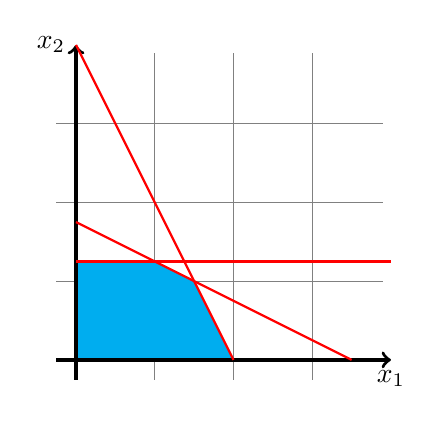
\begin{tikzpicture}[domain=0:4, align=center]
     \draw[very thin, color=gray](-0.25,-0.25) grid(3.9,3.9);
     \filldraw[fill=cyan, draw=red] (0,0) -- (0,1.25) -- (1,1.25) -- (1.5,1) -- (2,0) --  (0,0);
     \draw[very thick, ->] (0,-0.25) -- (0,4) node[left]{$x_2$};
     \draw[very thick, ->] (-0.25,0) -- (4,0) node[below]{$x_1$};
     
     \draw[thick, color=red] (0,1.75) -- (3.5,0);
     \draw[thick, color=red] (0,4) -- (2,0);
     \draw[thick, color=red] (0,1.25) -- (4,1.25);
   \end{tikzpicture}
   \end{center}
   
   \textbf{Corner Points}: 
   $$(0,0), (0,5), (0, 7), (0, 16), (8,0), (14,0), (4,5), (5.5,5), (6,4)$$
   
   \textbf{Feasible Corner Points}:
   $$(0,0), (0,5),  (8,0), (4,5), (6,4)$$
   
   \textbf{Objective Values for $\mathbf{z = 1000x_1 + 3000x_2}$}:
   $$z(0,0) = 0, z(0,5) = 15000, z(8,0) = 8000,$$
   $$z(4,5) = 19000, z(6,4) = 18000$$
   
   \textbf{Conclusion}: The most damage is dealt when Fireball is cast 4 times and Thunderbolt is cast 5 times. \newline{}
   
   (b) Changing Fireball's damage output to 2000 changes the objective function to
   $$z' = 2000x_1 + 3000x_2$$
   
  The constraints and feasible corner points of the problem remain the same.
  
   \textbf{Objective Values for $\mathbf{z' = 2000x_1 + 3000x_2}$}:
   $$z'(0,0) = 0, z'(0,5) = 15000, z'(8,0) = 16000,$$
   $$z'(4,5) = 23000, z'(6,4) = 24000$$
   
   \textbf{New Conclusion}: Now the most damage is dealt when Fireball is cast 6 times and Thunderbolt is cast 4 times.
   
   (c) While I do find it strange that a dragon will hold still while a wizard is bombarding it with fireballs and lightning bolts,
   while also not fighting back (which could affect the Certainty assumption as a wizard eaten by a dragon in 10 seconds won't really
   have the entire 32 seconds to cast spells for example.) an assumption that I find more questionable is the Divisibility assumption
   as it does not really make sense to partially cast a spell. 
   
   \textbf{Additional Comments}: Even though modelling this problem using integer programming may make more sense, in both (a) and (b),
   the optimum values for $x_1$ and $x_2$ were integers. Since the feasible region of the corresponding integer program is a subset of the
   linear program's feasible region, I think the optimum values of $x_1$ and $x_2$ for the integer program would be identical to those found
   for the linear program.
   
   Also, we need not be concerned with the Certainty assumption if the wizard is experienced enough so that none of the spells can miss and any damage
   done by the dragon is negligible. 
  \end{enumerate}
\end{document}